
\documentclass[12pt]{amsart}
\usepackage{geometry} % see geometry.pdf on how to lay out the page. There's lots.
\usepackage{graphicx}
\usepackage[]{algorithm2e}
\usepackage{amsmath}
\usepackage{subfig}
\usepackage{pdfpages}
\usepackage{floatrow}
\usepackage{parskip}
\usepackage{listings}
\usepackage{pythonhighlight}


\geometry{a4paper} % or letter or a5paper or ... etc
% \geometry{landscape} % rotated page geometry

% See the ``Article customise'' template for come common customisations

\title{SNACS - Extra Assignment}
\author{Steinar Bragi Sigurðarson}
\date{}

%%% BEGIN DOCUMENT
\begin{document}

\maketitle

\section{Exercise 1}

First we initalize our variables.

$W$ contains all vertices. Our global lower bound $\bigtriangleup_L = -\infty$ and $\bigtriangleup_U = \infty$


\textbf{Iteration 1:}\\
We start by looking at F because it has the highest degree.
We measure the eccentricity of F, $\varepsilon[v] = 5$.

We then update our global lower and upper bounds:

$\bigtriangleup_L = max(\bigtriangleup_L, \varepsilon[F]) = max(-\infty, 5) = 5$

$\bigtriangleup_U = min(\bigtriangleup_U, 2* \varepsilon[F]) = min(\infty, 2*5) = 10$

\begin{figure}[h]
\caption{Bounds after first iteration}
\centering
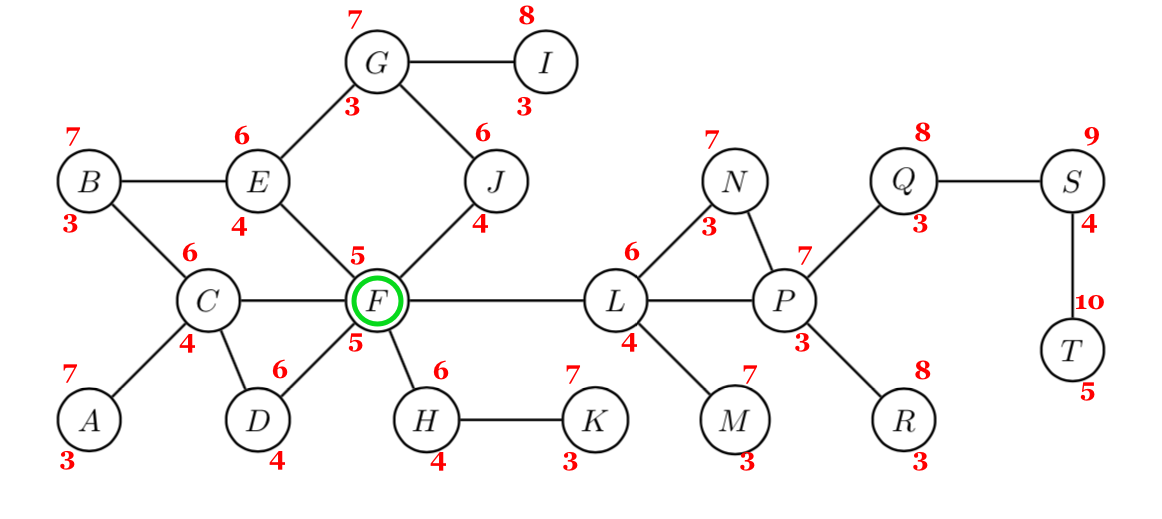
\includegraphics[width=0.8\textwidth]{iter1.png}
\label{iter1}
\end{figure}

For each node $w$ in $W$, including $F$ we measure upper and lower bounds as follows:

$\varepsilon_L[w] = max(\varepsilon_L[w],max(\varepsilon[v] - d(v,w),d(v,w)))$\\
$\varepsilon_U[w] = min(\varepsilon_U[w],\varepsilon[v] + d(v,w))$\\

In the case of $F$, that would give us the following upper and lower bounds:\\

$\varepsilon_L[w] = max(-\infty,max(5 - 0, 0)) = 5$\\
$\varepsilon_U[w] = min(\infty,5 + 0) = 5$\\

In the case of J, we would get:\\

$\varepsilon_L[w] = max(-\infty,max(5 - 1, 0)) = 4$\\
$\varepsilon_U[w] = min(\infty,5 + 1) = 6$\\

See figure ~\ref{iter1} for upper and lower bounds of all nodes after the first iteration.


During this iteration, $F$ will be discarded from $W$ because $\varepsilon_L[F] == \varepsilon_U[F]$


\textbf{Iteration 2:}\\
Next, we select a new node $v$ with the highest upper bound. In our case, it's $T$, with the following values:\\
$\varepsilon_L[w] = 10$\\
$\varepsilon_U[w] = 5$\\
We measure $v$'s eccentricity: $\varepsilon[v] = 8$\\
$\bigtriangleup_L = max(\bigtriangleup_L, \varepsilon[v]) = max(5, 8) = 8$ \\
$\bigtriangleup_U = min(\bigtriangleup_U, 2* \varepsilon[v]) = min(10, 2*8) = 10$

Again, for each node $w$ in $W$, including $T$ we measure upper and lower bounds. We also discard nodes from $W$ where $\varepsilon_L[F] == \varepsilon_U[F]$. Discarded nodes are circled in red in figure ~\ref{iter2}

\begin{figure}[h]
\caption{Bounds after second iteration}
\centering
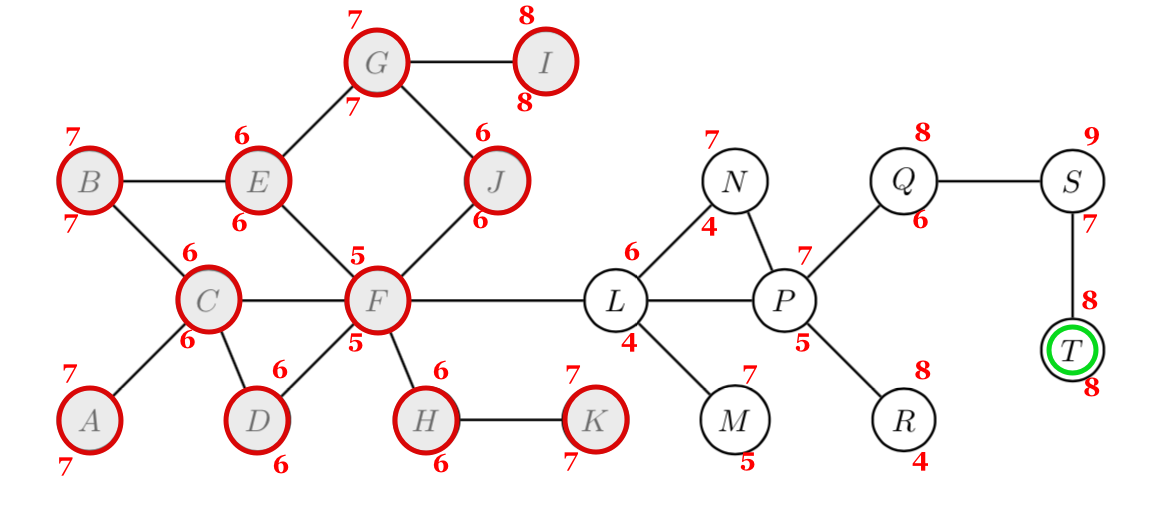
\includegraphics[width=0.8\textwidth]{iter2.png}
\label{iter2}
\end{figure}

\textbf{Iteration 3:}\\
Next, we select a new node $v$ with the lowest lower bound. In our case, $L$, $N$ and $R$ are tied with lower bounds of 4. $L$ has the highest degree, so we choose $L$ as our new $v$.\\
$v$'s eccentricity: $\varepsilon[v] = 4$\\

$\bigtriangleup_L = max(\bigtriangleup_L, \varepsilon[v]) = max(8, 4) = 8$ \\
$\bigtriangleup_U = min(\bigtriangleup_U, 2* \varepsilon[v]) = min(10, 2*4) = 8$ \\

\begin{figure}[h]
\caption{Bounds after third iteration}
\centering
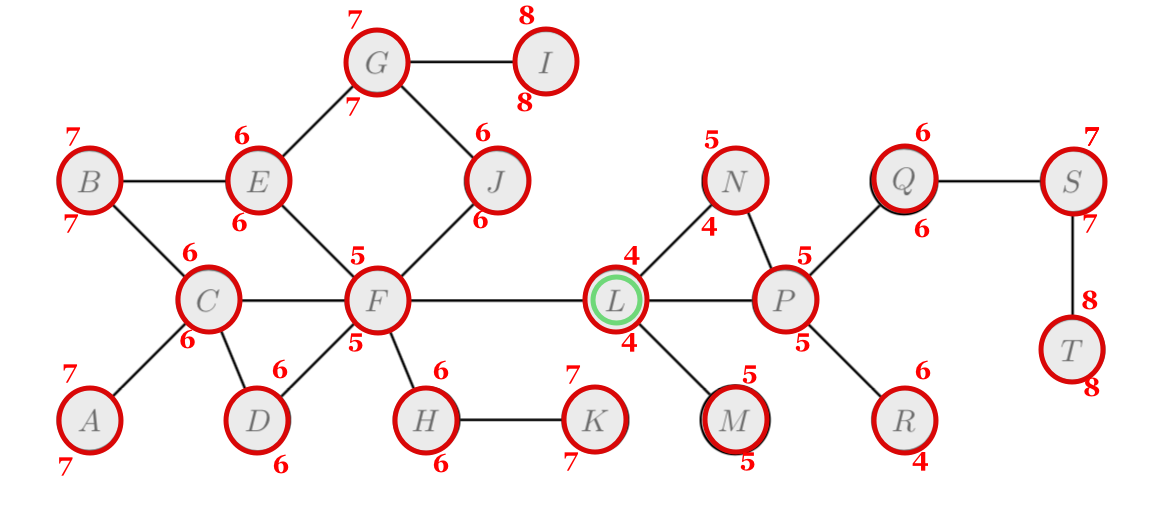
\includegraphics[width=0.8\textwidth]{iter3.png}
\label{iter3}
\end{figure}

As we can see from figure ~\ref{iter3}, all nodes have been discarded from $W$. \\ $\bigtriangleup_L = \bigtriangleup_U = 8$, so we conclude that the diameter of our graph is 8.

\section{Exercise 2}

For questions 2.1 - 2.5, I wrote python code using the following packages:

\begin{python}
import networkx as nx
import matplotlib.pyplot as plt
import numpy as np
\end{python}

Read the data from network.in with the read\_edgelist function from networkx:

\begin{python}
G=nx.read_edgelist("data/network.in",
create_using=nx.DiGraph(), nodetype=int)
\end{python}


\subsection{How many directed links does this network have?}

I call the following two networkx functions to get the number of edges (directed links) and nodes.

\begin{python}
print(G.number_of_edges())
\end{python}

The output is: \\
8070 \\

\subsection{How many nodes does this network have?}

Again, I used networkx.

\begin{python}
print(G.number_of_nodes())
\end{python}

The output, our number of nodes is: \\
1876 \\


\subsection{Give the indegree and outdegree distribution of this graph.}

I created a loglog plot of indegree and outdegree distribution with the following code:

\begin{python}
indegree = G.in_degree(G)
in_list = list(indegree.values())
in_values = sorted(set(indegree.values()))
in_hist = [in_list.count(x) for x in in_values]

outdegree = G.out_degree(G)
out_list = list(outdegree.values())
out_values = sorted(set(outdegree.values()))
out_hist = [out_list.count(x) for x in out_values]

plt.loglog(in_values,in_hist,'ro')
plt.loglog(out_values,out_hist,'b*')
plt.legend(['in-degree','out-degree'])
plt.ylabel('Occurrence')
plt.title('network.in loglog degree distribution')
plt.savefig('degreeloglog.png')
plt.show()
\end{python}

\begin{figure}[h]
\caption{In-degree and out-degree distribution of network.in}
\centering
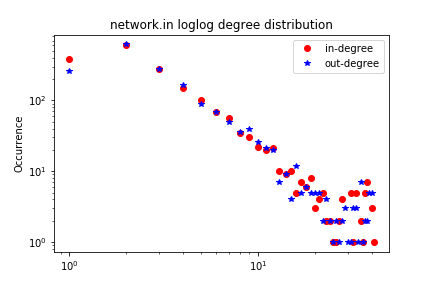
\includegraphics[width=0.7\textwidth]{degreeloglog.png}
\label{degreeloglog}
\end{figure}


\subsection{How many weakly connected components and how many strongly connected components does this network have? How many nodes and links are in the largest strongly connected component of this graph?}

I used the following functions:

\begin{python}
print('Weakly connected components: ',
  nx.number_weakly_connected_components(G))

print('Strongly connected components: ',
  nx.number_strongly_connected_components(G))
\end{python}

They gave me these results:\\
Weakly connected components:  5\\
Strongly connected components:  187


To find the number of links and nodes in the largest strongly connected component, I did this:

\begin{python}
ls = max(nx.strongly_connected_component_subgraphs(G),key=len)
print('LS num of edges: ', ls.number_of_edges())
print('LS num of nodes: ', ls.number_of_nodes())
\end{python}

The results are: \\
LS num of edges:  5220 \\
LS num of nodes:  1248

\subsection{Distance Distribution}

I iterate through all nodes in our largest strongly connected component. For each node, I find the distance to all other nodes. I then iterate through the resulting dictionary of distances (path lengths), increment the occurrences in my dist_hist dictionary which is indexed by distance values.
I then plot the distance indexed dictionary in a bar graph/histogram. The X axis shows distance values, Y shows their occurence.


\begin{python}
dist_hist = {}

for node in ls.nodes():
    dist_from_node = nx.single_source_shortest_path_length(ls,source=node)
    for k, v in dist_from_node.items():
        if v in dist_hist:
            dist_hist[v] += 1
        else:
            dist_hist[v] = 0

plt.bar(list(dist_hist.keys()), list(dist_hist.values()))
plt.xlabel('Distance')
plt.ylabel('Occurrence')
plt.title("Distance distribution of LSCC in network.in")
plt.savefig('distdist.png')
plt.show()
\end{python}

\begin{figure}[h]
\caption{Distance distribution of LSCC in network.in}
\centering
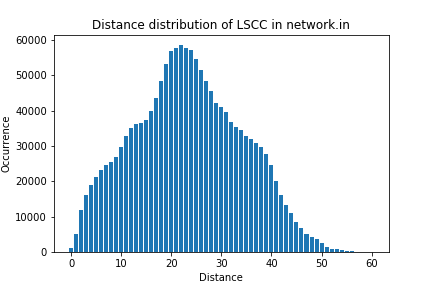
\includegraphics[width=0.7\textwidth]{distdist.png}
\label{distdist}
\end{figure}


\end{document}
